\section{Thảo luận}
\label{sec:discussion}

\subsection{SyscallAD đạt được gì so với công trình tham chiếu}
Về mặt thiết kế, SyscallAD tái hiện được \emph{định hướng} của lõi phát hiện DeSFAM:
một bộ phát hiện học một lớp (chỉ dùng dữ liệu lành tính) kết hợp lỗi tái cấu trúc
(VAE) với cô lập thống kê (iForest), trong đó các bit hiện diện syscall đặc quyền là
tín hiệu trực tiếp cho leo thang đặc quyền. Việc đánh giá ``tái lập thành công hay
chưa'' được căn theo tiêu chí đã cố định trước ở Mục~\ref{subsec:protocol} (ưu tiên
khả năng xếp hạng AUC/AP và định hướng precision, không lấy chênh lệch F1 tại một
ngưỡng làm phán quyết). Một điểm cần lưu ý: DeSFAM không công bố bảng AUC/AP/F1
theo mô hình trên DongTing (Mục~\ref{subsec:qual-ref}), nên ở đây \emph{không} có
phán quyết ``đạt/không đạt số liệu công bố theo mô hình''. Điều khẳng định được, một
cách trung thực, là: bản tái lập đạt khả năng \emph{xếp hạng} cao và ổn định (tập hợp
AUC $0{,}835$, AP $0{,}990$, $\pm 0{,}000$ qua hạt giống) và giữ định hướng \emph{ít
báo động giả} (precision $0{,}999$); còn recall/F1 thấp ($0{,}264$/$0{,}417$) là hệ
quả của ngưỡng \texttt{p995} và bảng chữ cái hẹp, không phải của năng lực xếp hạng.
So với mức \emph{tổng hợp} của DeSFAM (AUC $\approx 0{,}94$, F1 $\approx 0{,}92$),
AUC cùng tầm nhưng F1/recall thấp hơn---chênh lệch quy về ngưỡng và cấu hình.

\subsection{Ý nghĩa của khoảng cách ngưỡng và quản trị ngưỡng khi vận hành}
Với phát hiện bất thường, một mô hình \emph{xếp hạng} tốt (AUC/AP cao) vẫn có thể
cho F1 thấp tại một ngưỡng cố định nếu ngưỡng ưu tiên precision. Điều này cho thấy
giá trị của \emph{hiệu chỉnh ngưỡng theo môi trường}: ngưỡng nên được căn theo phân
phối điểm quan sát trong môi trường triển khai thay vì cố định từ tập kiểm định.
Số liệu xác nhận điều này: tại ngưỡng \texttt{p995}, precision đạt $0{,}999$ nhưng
recall mức cửa sổ chỉ $0{,}264$ (F1 $0{,}417$); gộp lên mức chuỗi, recall tăng lên
$0{,}338$ và F1 lên $0{,}502$. Khoảng cách so với F1 tổng hợp của DeSFAM ($\approx
0{,}92$) vì thế quy về \emph{chiến lược ngưỡng} (ưu tiên precision), không phải năng
lực xếp hạng---vốn cao và ổn định (AUC $0{,}835$, AP $0{,}990$).

\subsection{Lựa chọn thiết kế và phạm vi}
Báo cáo giới hạn không gian đặc trưng về 23 syscall an ninh---một bước \emph{chọn lọc
đặc trưng theo miền}, tập trung bộ phát hiện vào hành vi đặc quyền. Đánh giá được
thực hiện hoàn toàn ngoại tuyến trên DongTing; thành phần phục vụ trực tiếp cùng các
Mô-đun~1 và 3 của DeSFAM (lập danh sách seccomp, chấm điểm rủi ro, chặn trong nhân)
nằm ngoài trọng tâm và không được hiện thực hóa lại---báo cáo dừng ở mức phát hiện.

\subsection{Phản biện về ảnh hưởng của việc thu hẹp bảng chữ cái syscall an ninh}
\label{subsec:confound}
Một phản biện đáng lưu ý cần được xem xét: vì không gian đặc trưng giới hạn ở 23
syscall an ninh và khối lượng lành tính hầu như không gọi syscall đặc quyền, có thể nghi ngờ rằng
SyscallAD thực chất chỉ xác định \emph{sự hiện diện của một syscall đặc quyền} chứ
không thực sự phát hiện \emph{bất thường theo chuỗi}. Đây là một nguy cơ
\emph{nhiễu thiết kế} (confound) cần được thừa nhận. Ba lập luận làm giảm nhẹ---song
không loại bỏ hoàn toàn---phản biện này: (i) không phải syscall nào trong bảng chữ
cái cũng đặc quyền (\texttt{execve}, \texttt{openat}, \texttt{socket}, \texttt{mmap}
xuất hiện dày trong cả hai lớp), nên mô hình vẫn phải học cấu trúc cửa sổ chứ không
chỉ đọc một bit; (ii) đặc trưng \texttt{cat}/\texttt{stats}/\texttt{prefixspan} mã
hóa phân bố và tính tuần tự, không chỉ hiện diện; (iii) một số kỹ thuật leo thang
lạm dụng \emph{chính} các syscall hợp lệ (ví dụ chuỗi \texttt{execve} bất thường),
nơi bit hiện diện không đủ và mô hình chuỗi mới phân biệt được.

\paragraph{Kết quả thí nghiệm cắt bỏ.} Thí nghiệm cắt bỏ ``chỉ-\texttt{disc}'' cho
một kết luận phân đôi rõ ràng (Hình~\ref{fig:ablation}):
\begin{itemize}[leftmargin=1.6em]
  \item \textbf{Ở mức cửa sổ, phản biện có cơ sở.} Bộ đếm bit \texttt{disc} (chỉ
        biểu thị sự hiện diện của syscall đặc quyền) đạt AUC $0{,}875$, cao hơn cả
        tập hợp đầy đủ ($0{,}835$); $83{,}5\%$ cửa sổ tấn công chứa ít nhất một
        syscall đặc quyền. Ở mức cửa sổ, SyscallAD về cơ bản \emph{tương đương} một
        bộ phát hiện dựa trên hiện diện, phù hợp với phản biện nêu trên.
  \item \textbf{Ở mức chuỗi, mô hình có giá trị tăng thêm.} Khi gộp lên mức chuỗi,
        tập hợp đầy đủ đạt AUC $0{,}787$ trong khi chỉ-\texttt{disc} chỉ đạt
        $0{,}678$: cấu trúc cửa sổ mà VAE/iForest học được phân biệt tốt hơn đáng kể
        so với hiện diện đơn thuần, tại đơn vị vận hành thực (chuỗi/tiến trình).
\end{itemize}

\begin{figure}[htbp]
  \centering
  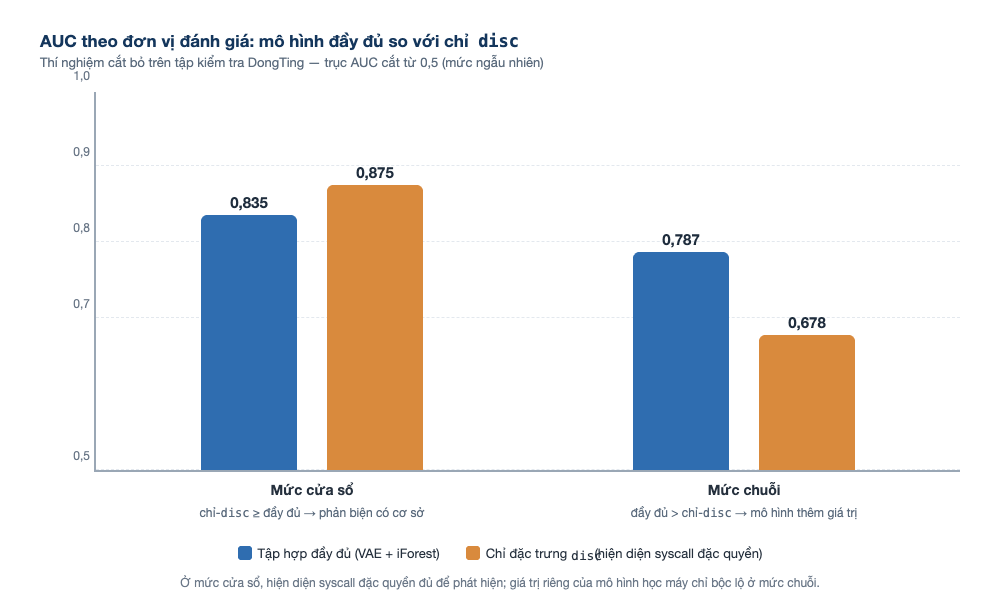
\includegraphics[width=\linewidth]{figures/ablation-auc}
  \caption{Thí nghiệm cắt bỏ trên tập kiểm tra DongTing: AUC của tập hợp đầy đủ
           (VAE\,+\,iForest) so với bộ phân loại chỉ dùng đặc trưng \texttt{disc}.
           Ở \emph{mức cửa sổ}, chỉ-\texttt{disc} ($0{,}875$) ngang bằng hoặc cao
           hơn mô hình đầy đủ ($0{,}835$)---phản biện ``đường tắt theo hiện diện'' có
           cơ sở. Ở \emph{mức chuỗi}, mô hình đầy đủ ($0{,}787$) vượt rõ chỉ-\texttt{disc}
           ($0{,}678$)---mô hình học máy đóng góp giá trị vượt trên hiện diện đơn thuần.}
  \label{fig:ablation}
\end{figure}

Như vậy, tại đơn vị cửa sổ, năng lực phát hiện phần lớn quy về sự hiện diện của
syscall đặc quyền; giá trị riêng của mô hình học máy chỉ bộc lộ ở mức chuỗi. Do đó
báo cáo \emph{không} khẳng định ``cơ chế bất thường theo chuỗi vượt trội'' một cách
tổng quát mà giới hạn kết luận ở mức chuỗi, đồng thời đề xuất bổ sung khối lượng lành
tính có gọi syscall đặc quyền hợp lệ (chẳng hạn trình gỡ lỗi, hoặc sidecar quan sát
sử dụng \texttt{bpf}) để kiểm chứng chặt chẽ hơn.

\paragraph{Đối soát mã hóa (cảnh báo từ kiểm toán).} Kiểm toán đối soát mã hóa phát
hiện $2/24$ syscall trong bảng chữ cái (\texttt{setgid}, \texttt{unlinkat}) xuất
hiện trong chuỗi lành tính (mã ID) nhưng \emph{vắng mặt} trong chuỗi tấn công (mã
tên). Đây có thể là bất đối xứng tự nhiên hoặc một \emph{lệch ánh xạ tên\,$\to$\,ID}
cần điều tra (ví dụ tên thay thế như \texttt{setgid32}, \texttt{unlink}); nếu là
lệch ánh xạ, các bit \texttt{disc} tương ứng sẽ bật bất đối xứng giữa hai lớp---một
hạng mục cần kiểm tra trước khi diễn giải sâu hơn.

\subsection{Hạn chế và đe dọa tính hợp lệ}
\begin{itemize}[leftmargin=1.6em]
  \item \textbf{Hợp lệ nội tại:} đánh giá dựa trên các chuỗi syscall của DongTing
        (chương trình kích hoạt lỗi nhân), không phải vết khai thác CVE thực thi
        đầu-cuối; kết quả phản ánh khả năng phân biệt trên dữ liệu này.
  \item \textbf{Hợp lệ ngoại tại:} DongTing là chuỗi lỗi nhân, có thể chưa đại diện
        đầy đủ cho hành vi container/khối lượng công việc sản xuất; cần mở rộng nguồn
        dữ liệu để khái quát hóa.
  \item \textbf{Hợp lệ kết luận:} mất cân bằng lớp lớn khiến AP dễ gây hiểu nhầm; cần
        báo cáo kèm AUC, precision, recall để tránh kết luận một chiều.
  \item \textbf{Hợp lệ cấu trúc:} đặc trưng thời gian bị tắt do DongTing không có dấu
        thời gian theo syscall; mô hình có thể thiếu một tín hiệu mà công trình tham
        chiếu tận dụng.
  \item \textbf{Nhãn mức cửa sổ:} việc kế thừa nhãn chuỗi xuống mọi cửa sổ
        (Mục~\ref{subsec:protocol}) gán nhãn ``tấn công'' cho cả các cửa sổ lành tính
        bên trong chuỗi tấn công, làm lệch AUC/AP/F1; đây là lý do báo cáo kèm chỉ số
        mức chuỗi.
  \item \textbf{Tấn công thích nghi:} mô hình đe dọa giả định tấn công bộc lộ syscall
        đặc quyền; một kẻ tấn công biết bảng chữ cái 23 lời gọi có thể \emph{bắt
        chước} (mimicry~\cite{wagner2002mimicry}) hành vi lành tính hoặc pha loãng để
        tránh bật bit \texttt{disc}. Công trình gần đây xác nhận bộ phát hiện theo
        chuỗi vẫn bị né tránh bằng tiêm đối kháng kiểu seqGAN và đề xuất hướng tăng
        cường độ bền vững~\cite{advrobustseq2025}. Đây là giới hạn cố hữu của phát
        hiện dựa trên hiện diện và là hướng cần đánh giá đối kháng.
\end{itemize}
